% This is samplepaper.tex, a sample chapter demonstrating the
% LLNCS macro package for Springer Computer Science proceedings;
% Version 2.20 of 2017/10/04
%
\documentclass[runningheads]{llncs}
%
\usepackage{graphicx}
% Used for displaying a sample figure. If possible, figure files should
% be included in EPS format.
%
% If you use the hyperref package, please uncomment the following line
% to display URLs in blue roman font according to Springer's eBook style:
% \renewcommand\UrlFont{\color{blue}\rmfamily}
\usepackage[ruled,vlined,linesnumbered]{algorithm2e}

\begin{document}
%
\title{Automatic Generation and Translation of Process Collaboration Models}
%
%\titlerunning{Abbreviated paper title}
% If the paper title is too long for the running head, you can set
% an abbreviated paper title here
%
\author{Frederik Bischoff \and Walid Fdhila}

%\author{Frederik Bischoff\inst{1} \and Walid Fdhila\inst{1}}
%
\authorrunning{F. Bischoff et al.}
% First names are abbreviated in the running head.
% If there are more than two authors, 'et al.' is used.
%
\institute{Faculty of Computer Science, University of Vienna, Austria}
%
\maketitle              % typeset the header of the contribution
%
\begin{abstract}
In the research field of business process models and techniques, researchers can only rely on a repository of centralized, intra-organizational processes to use as support of their work. But regarding decentralized, cross-organizational models, they face the problem that there is a lack of available model examples. Within this work this lack is tried to be tackled. Thereby, a concept is introduced how to generate collaborative business processes randomly by following a \textit{top-down approach}, which first generates the choreography model and then derives the public and private models of each process participant from it. Additionally, a possibility for specifying and imposing global compliance rules onto the collaboration is elaborated. The conception of this random collaboration process generator is prototypically implemented within an existing framework in order to evaluate the process. During the generation, the models are maintained as a Refined Process Structure Tree. In order to utilize the generated processes for the support of for further research, the models are exported in BPMN notation.  

\keywords{Process Collaboration  \and Automatic Generation \and Process Models \and Compliance Rules.}
\end{abstract}
%
%
%
\section{Introduction}
In the research field of business process models and techniques, researchers can only rely on a repository of centralized, intra-organizational processes to support their work. But regarding decentralized, cross-organizational models, they face the problem that there is a lack of available model examples. Within the scope of this work, this lack is aimed to be tackled. Thereby, the main objective is to build a repository of distributed and collaborative process models by developing and implementing an automatic generation process for business process collaborations. The generation process must thereby ensure soundness, consistency and compatibility of the resulting models. Additionally, it should also allow the generation of models which comply to imposed compliance rules. At last, to ensure the executability of the auto-generated models by process engines, an additional goal of this work is to develop a transformation of the utilized RPST\footnote{Refined Process Structure Tree } representation to BPMN\footnote{Business Process Model and Notation - http://www.bpmn.org/}. These requirements ensure that the repository can then be used for further research, such as change management or process mining of collaborative processes. Based on those objectives, the following research questions are derived:

\begin{itemize}
\item \textit{RQ-1}: How to build a repository of collaboration process models that can be used as support for further research in this field?
\item \textit{RQ-2}: How to ensure that the resulting process models in this repository are correct in terms of consistency, compatibility and compliability? Which process flow perspectives and compliance rule patterns should be supported regarding compliability? 
\item \textit{RQ-3}: How to transform a collaborative process represented as an RPST into an executable form?
\end{itemize}

This work is part of the CRISP\footnote{http://gruppe.wst.univie.ac.at/projects/crisp/} project (ICT15-072) funded by the Vienna Science and Technology Fund (WWTF). The implementation of the prototype is integrated in an already existing framework. The main research within the project is to analyze flexibility and adaptivity of collaborative business processes at design time as well as at runtime. Regarding consistency and correctness of collaborative business processes, the propagation of a process change over all process participants is one of the main challenges the project tries to tackle. Furthermore, the impact of compliance rules imposed on collaborative business scenarios is analyzed as well as the issue of ensuring business compliance by considering the privacy and autonomy of the involved business partners.\\

This work is structured as followed. First, a brief blablabla.

\section{Process Collaborations} % short introduction into process collaborations and the three levels of correctness
This chapter provides the basics of business process collaborations, represented in BPMN. In BPMN, collaborative processes are represented from different perspectives, whereas each perspective is represented by a different BPMN model type. In the following, the different model types and their represented perspective are explained with the help of a collaborative business process example.

\subsection{Different Perspectives of Process Collaborations}
Blablabla... TODO: smaller and simpler example collaboration

\subsubsection{Private Model}
The private model is modeled from the perspective of a single participant of a collaborative process. In a collaborative scenario, it describes the complete internal business logic of one partner as well as the messages exchanged with other partners. Activities which are only for the participant are called \textit{private activities}, whereas activities which involve participation of other partners are called \textit{public activities}.\\

\begin{figure}
\centering
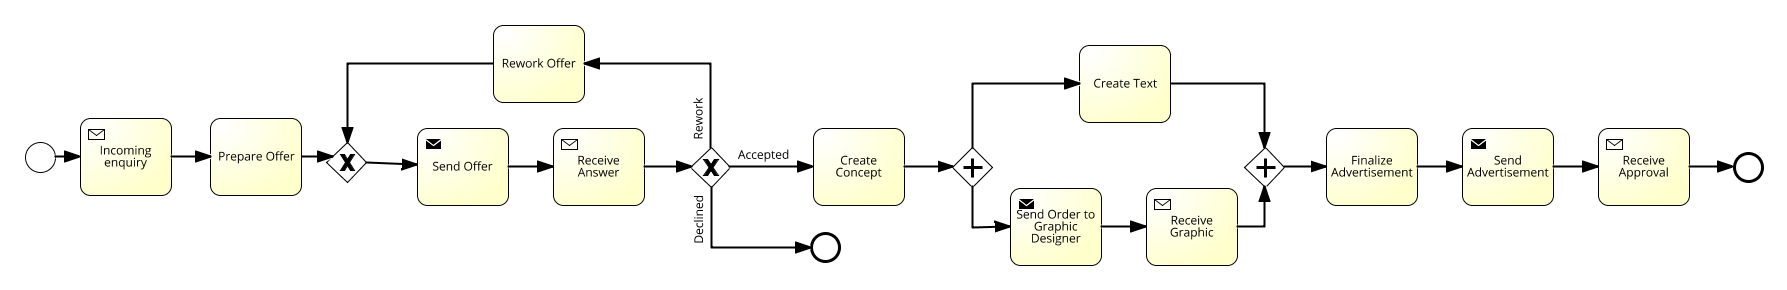
\includegraphics[width=\textwidth]{images/private_process_agency.png}
\caption{Private Model Example}
\label{fig:privateModel}
\end{figure}

For example, in the private model shown in Figure \ref{fig:privateModel}, the task \textit{Create Concept} represents a private activity, whereas the task \textit{Send Offer}, involves message exchange with another participant and therefore represents a public activity. A private model is a process model in the classical sense. It's fundamental modeling objects are unchanged since BPMN 1.0. Is a private process modeled and attributed in detail, it also represents an executable process that can be executed by a process engine.

\subsubsection{Public Model}
The public model is also modeled from the perspective of a single participant of a collaborative process. It is a reduced view on the private model of a partner. It can also be described as a projection of the whole collaboration process focusing on one participant. It only includes public activities, involving message exchange with other partners. Private activities which are not relevant for other partners and which don't want be to be shared with the partners are omitted deliberately. Figure \ref{fig:publicModel} shows the corresponding of the already introduced private model. 

\begin{figure}
\centering
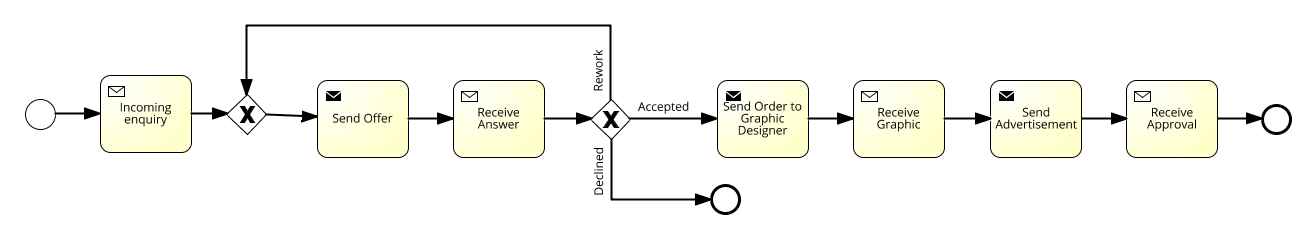
\includegraphics[width=\textwidth]{images/public_process_agency.png}
\caption{Public Model Example}
\label{fig:publicModel}
\end{figure}

\subsubsection{Collaboration Model}
The collaboration model is the interconnection between the public models of all participants. The thereby formed model gives a holistic view on the collaborative process and does not focus on one partner. Each partner is represented as a pool and the message exchange between them is shown by a message flow that connects two public activities or just the pools. Figure \ref{fig:collabModel} shows an example collaboration model.

\begin{figure}
\centering
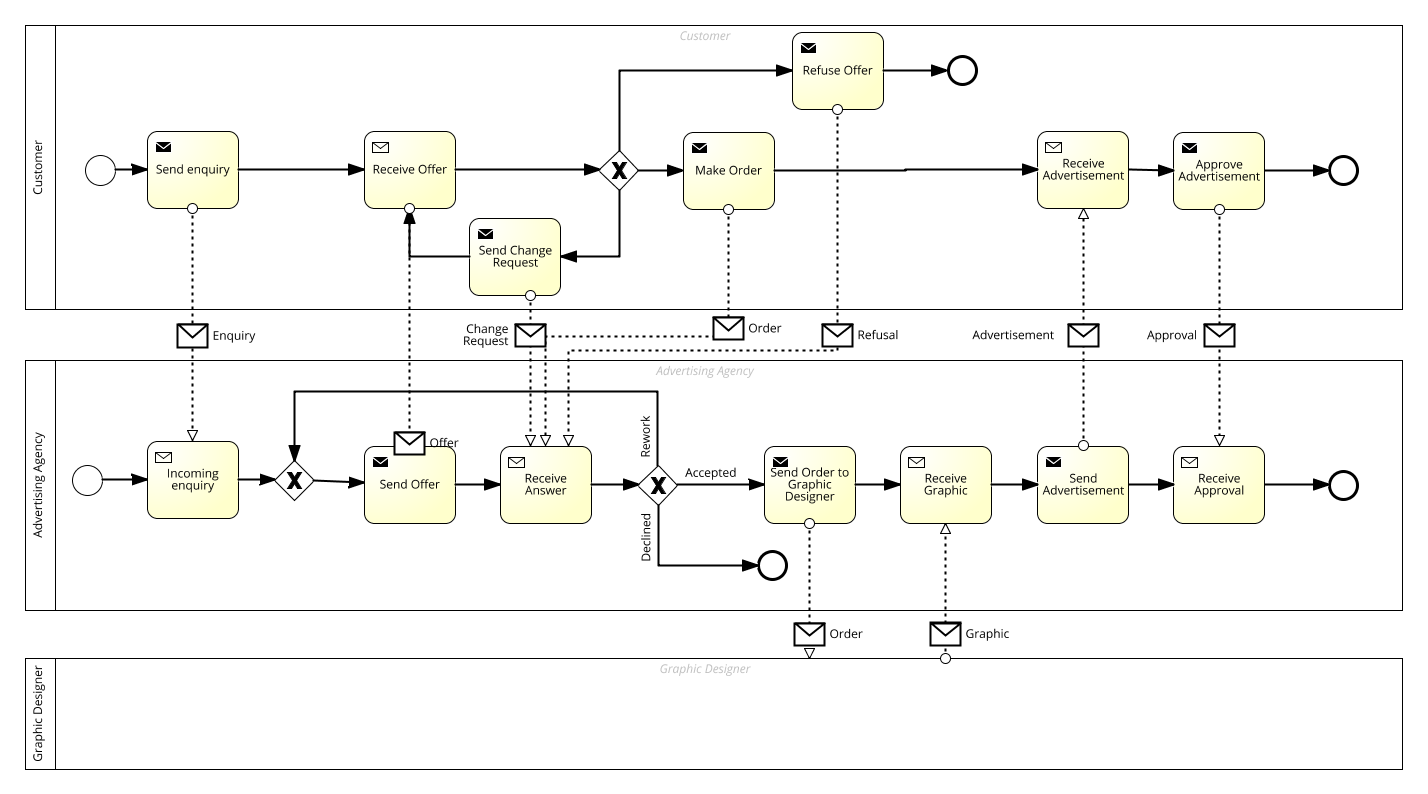
\includegraphics[width=\textwidth]{images/collab_advertisement.png}
\caption{Collaboration Model Example}
\label{fig:collabModel}
\end{figure}

Each partner's public process is modeled inside a pool. It is also allowed for a process to not include the public model inside an participant's pool. If a pool contains a process, it is called a "white box". If a pool is empty, it's called a "black box". For Example in figure \ref{fig:collabModel} the pools of the partners \textit{Customer} and \textit{Advertisement Agency} are modeled as "white box" and the pool of the \textit{Graphic Designer} as a "black box" \cite{BPMN20}.

\subsubsection{Choreography Model}
The choreography model is available since BPMN 2.0 and focuses solely on the sequence of message exchanges between the partners. Each message exchange is represented as an interaction with an initiating 
partner, a receiving partner (shaded in grey) and the message exchanged. In contrast to the collaboration model, which also focuses on the message flow, the choreography model additionally displays the exact sequence flow (i.e. conditional message flows or parallel message flows), which is not always evident form the former (i.e. black box pools).

\begin{figure}
\centering
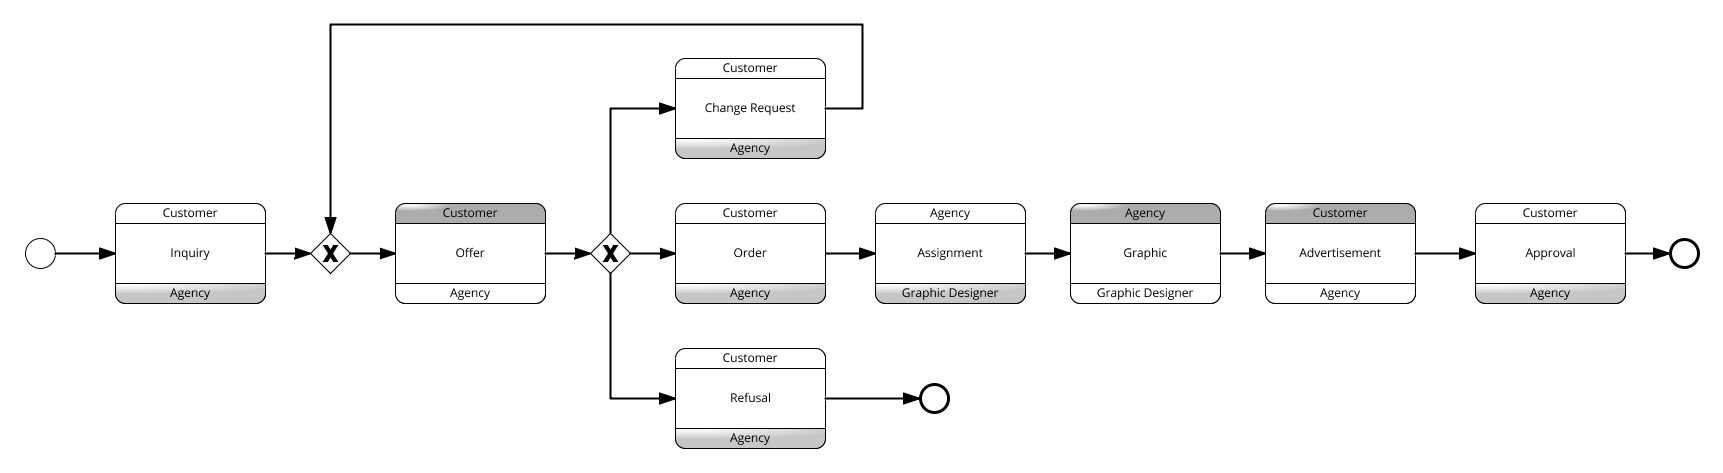
\includegraphics[width=\textwidth]{images/choreo_advertisement.png}
\caption{Choreography Model Example}
\label{fig:choreoModel}
\end{figure}

\subsection{Correctness Levels of Process Models}
maybe just cite \cite{sabrina848}

\section{Automatic Collaboration Generation Approach}

\subsection{Top-Down Approach}
As already mentioned, a process collaboration involving several partners can be modeled from different perspectives (partner or global) through the use of different model types. The process collaboration generator, implemented in the context of this work, generates all three different model types as the output. In general, there exist two different approaches to build a process collaboration with all the described models \cite{sabrina1174}. In the \textit{top-down approach}, first the choreography model is build, then the public and private models of each partner are derived and defined consistently. In comparison, in the \textit{bottom-up approach}, each partner has already defined a private and public process. Then, the choreography model is constructed by connecting the public models via message exchange. The automatic generator process, presented in this work, follows the \textit{top-down approach}, by first generating the choreography model and then deriving the collaboration, public and private models from it. Thereby, each interaction (choreography task) of the choreography model is converted into a send and receive task and then added to the involved partners processes, to build their public process models. In turn, each private model is derived from its corresponding public model by enriching the public model with abstract private tasks. The collaboration model is then built by composing the partner's public processes into one model.

\begin{figure}
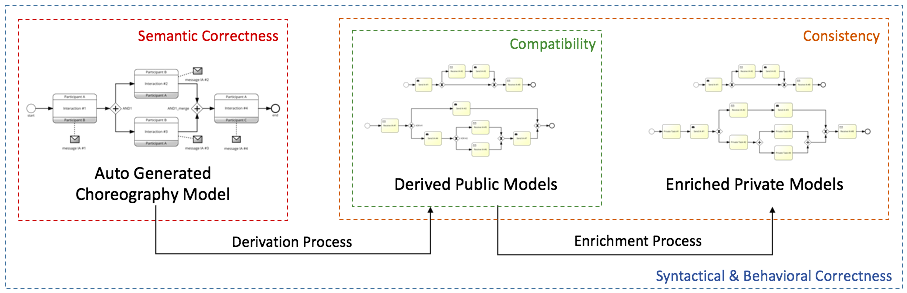
\includegraphics[width=1\textwidth]{images/conception_approach.png}
\caption{Top-Down Approach}
\label{fig:topdownapproach}
\end{figure}

All three correctness levels are considered by the proposed algorithm for implementing an automatic process generator. The algorithm ensures that only model specific flow objects are used to build the processes and that they are connected appropriately (syntactical correctness). It also guarantees the absence of deadlocks and lifelocks (behavioral correctness) and offers the possibility to define global compliance rules, to which the generated collaboration should comply (semantic correctness). Deriving all models from the before generated choreography model offers also the advantage, that if the deriving process is implemented correctly, it already ensures \textit{consistency} and \textit{compatibility} between the different models. In the context of collaborative processes, \textit{consistency} means, that the private model of a partner has to be consistent with the corresponding public model, whereas \textit{compatibility} requires the public models of the collaborating partners to be compatible with one another \cite{FDHILA20151}. This ensures that the executed business process of one partner satisfies the behavior that is communicated to the partners through his public models \cite{sabrina1174}.

\subsection{Constraining the Collaboration}

Despite the premise that the process collaborations should be generated randomly, it is reasonable to set some boundaries within which the random generation takes place. The implemented generator provides two different ways to influence the resulting choreography model and hence the whole collaboration. The first one provides the possibility to constrain the choreography model in terms of the employed flow objects and their exact quantity by specifying several input parameters. The second one enables the user to impose global compliance rules based on compliance patterns to which the resulting model must comply.

\subsection{Parametric Constraints} \label{sec:param_constraints}

The following input parameters are specified to influence the random generation of the choreography model and hence also the deriving models:

\begin{itemize}
\item Number of Partners: \\Determines the number of participants that are involved in the process collaboration.
\item Number of Interactions: \\Determines the number of messages that are exchanged between the partners.
\item Number of Exclusive Gateways: \\Determines the number of Exclusive Gateways that are put into the model.
\item Number of Parallel Gateways: \\Determines the number of Parallel Gateways that are put into the model.
\item Max. Branching: \\Determines the maximum possible number of paths created for each gateway.
\end{itemize}

\subsection{Compliance Constraints} \label{sec:conception_compliance}

Generally, compliance rules can be defined for different process flow perspectives of a process. It can be distinguished between compliance rules that constrain the control flow (sequence of activities), the data associated with the activities, the resources (specific user or role) that perform the activities or the time perspective. There exist several languages and approaches on how to define and specify compliance rules, including formal languages \cite{Ghose2007},\cite{GovMilSad:edoc:06:compliance}, visual languages \cite{sabrina953},\cite{Awad2008} and pattern-based approaches \cite{compliance_patterns}, \cite{Ramezani2012}. Both visual and pattern-based approaches aim at hiding formal details (e.g. temporal logic) and therefore simplifying the specification of compliance rules. \\

For the specification of compliance rules for the automatic process generator, the pattern-based approach of Turetken et. al. \cite{compliance_patterns} is utilized. In \cite{compliance_patterns} a repository of \textit{process control patterns} is introduced, which are high-level templates used to represent process properties which the process specification must satisfy. Because the generated process collaborations neglect the data, time and resource perspective and focus solely on the control flow, only compliance rules that constrain the sequence of activities are possible to impose. Following process control patterns are supported to constrain the automatic generated choreography:

\begin{table}[]
\centering
\resizebox{12cm}{!}
{
\begin{tabular}{l|l}
Pattern		      & Description  \\ \hline
P LeadsTo Q       & Interaction P must lead to Interaction Q	  	 \\
P Precedes Q      & Interaction Q must be preceded by Interaction P	  \\
P Exclusive Q     & Interaction Q .. (not yet implemented!!!) \\ 		
P Universal  	  & Interaction P must always occur throughout execution \\
P Exists		  & Interaction P must be specified in process \\
\end{tabular}%
}
\caption{Overview of supported Compliance Patterns}
\label{tab:compl_patterns}
\end{table}

Note that the \textit{P LeadsTo Q} pattern does not demand an immediate succession of interaction Q on interaction P.

\subsection{Random Process Generation}
In this chapter, the needed components and their functionality for implementing a random process generator are explained. Each component encapsulates a step of the above described approach. Based on this approach, four components with single responsibilities can be derived: one component is responsible for randomly generating a choreography model, one for imposing compliance rules on the resulting process, another for deriving the remaining model types and the last component keeps control over the overall process. In the following the components and their functionalities will be explained in details.

\subsection{Overall Generation Process} \label{sec:overallprocesscontroller}
The \textit{Overall Process Controller} represents the orchestration component for building random process collaborations, based on given constraints. The process follows the principle \textit{'first build then check'}, which means that after a random choreography model has been generated, it will then be checked if the interactions defined within the compliance rules, can be assigned into the already built model in such a way that the resulting interaction sequence complies to the imposed rules. If the interaction allocation is not possible without violating the compliance rules, new random models will be build until a compliant model has been generated. If the imposing of the compliance rules fails repeatedly, it's an indicator that the amount of interactions in the model is too small relative to the unique interactions specified within the compliance rules. To overcome this, the number of interactions is increased by 10 percent every 10th build. After a successful assignment of the compliance rules, the remaining public and private models are derived out of the generated choreography model. At last, all models will be translated into a valid BMPN/XML.






%
% ---- Bibliography ----
%
% BibTeX users should specify bibliography style 'splncs04'.
% References will then be sorted and formatted in the correct style.
%
\bibliographystyle{splncs04}
\bibliography{bibliography}
%
\end{document}
